%******************************************************************************%
%                                                                              %
%                  sample.en.tex for LaTeX                                     %
%                  Created on : Tue Mar 10 13:27:28 2015                       %
%                  Made by : David "Thor" GIRON <thor@42.fr>                   %
%                                                                              %
%******************************************************************************%

\documentclass{42-en}


%******************************************************************************%
%                                                                              %
%                                    Header                                    %
%                                                                              %
%******************************************************************************%
\begin{document}



                           \title{Structured Query Language: Intermediate!}
                          \subtitle{Beating a dead horse}
                       \member{Ted Tran}{ttran@student.42.us.org}
                        \member{42 figment of your imagination}{pedago@42.fr}

\summary {
  This project is the sequel to "Introduction to \texttt{SQL}".
}

\maketitle

\tableofcontents


%******************************************************************************%
%                                                                              %
%                                  Foreword                                    %
%                                                                              %
%******************************************************************************%
\chapter{Foreword}

\texttt{Zoomer}: \\
Refers to members of Generation Z and is a play on the term "Boomer," which refers to members of the Baby Boomer generation. The term Zoomer is also in reference to the fast-paced upbringings members of Generation Z are characterized to have due to the fast advances in technology and culture that has been happening around them as a result of the interconnectivity of the American and Global populations because of the ubiquity of internet-connected smart phones and social media.

Example of use in sentence: "I can't stand those Zoomers, all they do is use their phones all day to play Fortnite and watch TikTok videos!"

From \href{https://www.urbandictionary.com/define.php?term=Zoomer}{urbandictionary}.
    % Spacing in the source code does not influence spacing in the
    % generated pdf. The blank lines aboves and below won't appear.
    % Instead, use \newline (or its shortcut \\) and \newpage to
    % create vertical spacing.
    
            \begin{figure}[H]
                \begin{center}
                    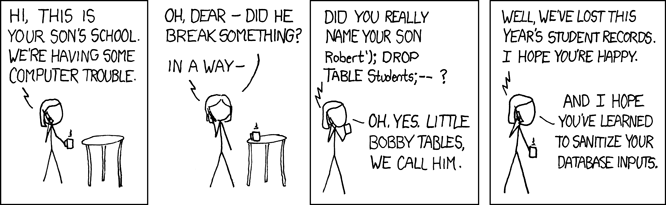
\includegraphics[width=17cm]{exploits.png}
                \end{center}
            \end{figure}

	    From xkcd! \\
	    	\newpage 	

%******************************************************************************%
%                                                                              %
%                                 Introduction                                 %
%                                                                              %
%******************************************************************************%
\chapter{Introduction}

	What the hell am I going to be doing?

	\begin{itemize}\itemsep1pt
		\item First, you're going to be running a ton of docker commands 
			so that you can run various things on these 42 lab computers
		\item Next, you're going to be building upon the SQL fundamentals you've learned. 
			You'll be reinforcing your fundamentals as well as building ontop of it. 
		\item Mhm, as usual it's time to write a ton of queries. Skill through experience!   
		\item Well, this time around, you'll be learning how to create your own database. 
			So, guess what the end goal is?
		\item You're going to create your own database! 
		\item After creating your database, you'll be filling it with data that you'll get 
			from web scraping, APIs, randomly generated, or just added manually.
		\item Then finally, it's time for you to create a wrapper so users can interact 
			with your database without writing SQL queries themselves. 
	\end{itemize}


	Testing is provided for you, so you only need to run a single command to 
	check your answers! Go for the green, buddy. 

%******************************************************************************%
%                                                                              %
%                                  Goals                                       %
%                                                                              %
%******************************************************************************%
\chapter{Goals}

	\begin{itemize}\itemsep1pt 
		\item Reinforce SQL fundamentals
		\item Learn MORE SQL, because this is a SQL project after all
		\item Learn how to create a database in Postgresql or Sqlite3
		\item Then use what you've learned at H2S to fill the database with... data!  
		\item Create a wrapper using a programming language of your choice, so 
			that a person can obtain information from your database without 
			having to write SQL queries themselves.
	\end{itemize}

	Your goal is to pass every single test for a beautiful 100 percent GREEN. Then 
	after that, use what you've learned at H2S to create your own database, seed it 
	with data, and create methods so users can interact with your DB without writing SQL queries! 

%******************************************************************************%
%                                                                              %
%                             General instructions                             %
%                                                                              %
%******************************************************************************%
\chapter{General instructions}

	\begin{itemize}\itemsep1pt 
		\item This project will be corrected by humans only. 
			You're allowed to organize and name your files as you see 
			fit, but you must follow the following rules. 
		\item The first rule of SQL Club is: You do not talk about SQL Club.
		\item The second rule of SQL Club is: You do not ta... wait, we did this already last time. 
			Well, this project's subtitle is beating a dead horse after all. 
		\item Within the mandatory part, you are only allowed to use SQL. 
		\item You can ask your questions on slack and random people in your nearby vicinity 
			that appear to be older than you. Of course, with the exception being me-- don't ask me 
			any questions. Everybody at 42 is a SQL master, and H2S mentors are required 
			to have a PhD in Structured Query Language studies! So don't be afraid to 
			come to them for guidance.
		\item The people who refused to give you help in the previous course were merely lazy. They dared to lie to your 
			face and say, "I don't know SQL!" so they could avoid helping you. Come after them with renewed vigor! 
		\item You will be provided with instructions on how to setup your programming environment, create the DB 
			and import data, a skeleton to code in, and a full testing suite to check your answers.
	\end{itemize}

% Don't forget this line for piscine days to initate the exercise counter at 0
\startexercices

%******************************************************************************%
%                                                                              %
%                             THE SQL PISCINE LOL                              %
%                                                                              %
%******************************************************************************%

\chapter{Day \exercicenumber: We meet again, young one }

\extitle{SQL Logical Order, .schema/.table, DB basics}
\exfiles{movie\_sql.rb}
\exnotes{Make sure to use docker cp to store your files on the host computer, then add it to a git repo after!}
\makeheaderfiles

	In case you're wondering... you'll be doing Assignment 1 on day00, Assignment 2 on day01, Assignment 3 on 
	day 02, then there's no Assignment 4 because 4 is a really unlucky number. You got lucky there, kiddo. 
	Notice how both PDFs end on day03? \\

	\begin{itemize}\itemsep1pt 
			\item	Read this! \href{https://blog.jooq.org/2016/12/09/a-beginners-guide-to-the-true-order-of-sql-operations/}{SQL logical order isn't the same as its syntactic order!}
		\item Look over the import\_db.sh script and the import\_db.sql to see how to create, delete, and import 
			databases in SQLite3.
		\item Creating and deleting databases in SQLite is different from PSQL-- why is this? Hint: 
			it's because SQLite has an embedded database-- the database is simply a normal file within 
			the computer's file system. 
		\item What if you want to view the database schema without looking at the import\_db.sql file? Look at the 
			example below!

	\end{itemize}
 
            \begin{figure}[H]
                \begin{center}
                    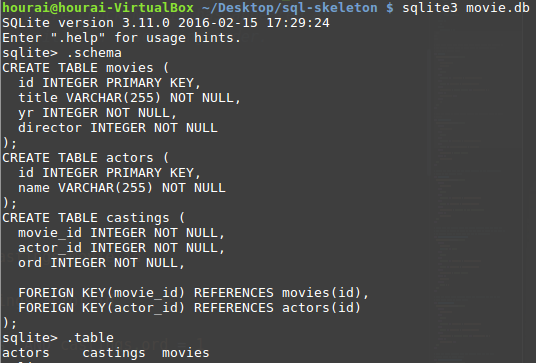
\includegraphics[width=14cm]{schema.png}
                \end{center}
            \end{figure}

	Eh. When writing queries in SQLite3, end them with ";" or they won't work. Use ".q" to exit out! \\ 
	


% Don't forget this line in order to increment the exercise counter
\nextexercice

%******************************************************************************%
%                                                                              %
%                             THE SQL PISCINE LOL                              %
%                                                                              %
%******************************************************************************%

\chapter{Day \exercicenumber: Damn, you're getting old }
\extitle{Pagination, subqueries into joins, and insert/update/delete}
\exfiles{movie\_sql.rb}
\exnotes{Make sure to use docker cp to store your files on the host computer, then add it to a git repo after!}
\makeheaderfiles

	\begin{itemize}\itemsep1pt
		\item What is pagination?! And why is keyset pagination almost always the better choice than offset pagination?
			\href{http://allyouneedisbackend.com/blog/2017/09/24/the-sql-i-love-part-1-scanning-large-table/}{Here 				is a good ol' example of keyset pagination vs offset}
		\item \href{https://academy.vertabelo.com/blog/converting-subqueries-joins/}{Converting subqueries to joins for better performance and cleaner code!}
		\item Basically, you'll want to have joins replace correlated subqueries if possible. 
		\item Look at the example below on how to insert, update, and delete rows in SQLite3! 
	\end{itemize}

            \begin{figure}[H]
                \begin{center}
                    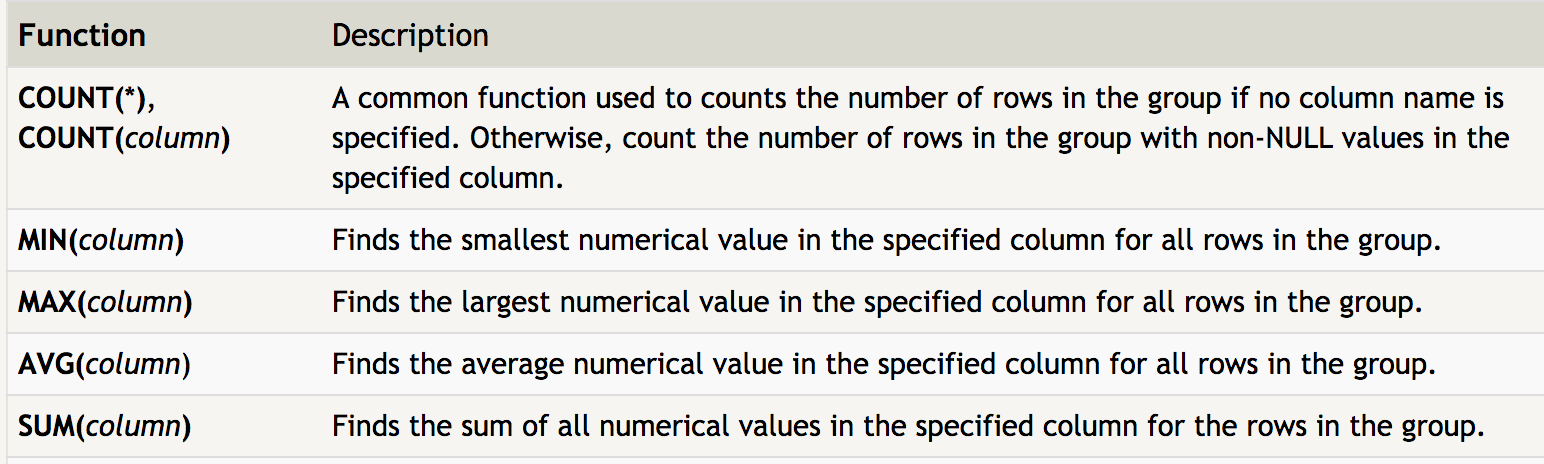
\includegraphics[width=14cm]{aggregate_functions.png}
                \end{center}
            \end{figure}

% Don't forget this line in order to increment the exercise counter
\nextexercice

%******************************************************************************%
%                                                                              %
%                             THE SQL PISCINE LOL                              %
%                                                                              %
%******************************************************************************%

\chapter{Day \exercicenumber: I miss the good old days... I remember when you were just a wee lad }

\extitle{Union/Intersect/Except, indexing, sanitization, constraints, table altering}
\exfiles{nonexistent\_sql.rb}
\exnotes{Make sure to use docker cp to store your files on the host computer, then add it to a git repo after!}
\makeheaderfiles

            \begin{figure}[H]
                \begin{center}
                    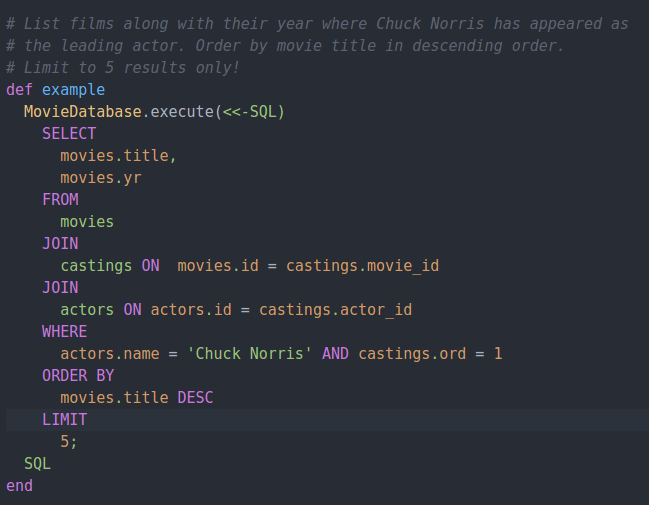
\includegraphics[width=13cm]{join.png}
                \end{center}
            \end{figure}

	\begin{itemize}\itemsep1pt 
		\item Above, example of Union/Intersect/Except with explanation of what's happening on each here 
		\item After that, some information about indexing + sanitization + constraits here 
		\item After that, an example below about how to alter a table in SQLITE3
	\end{itemize}

            \begin{figure}[H]
                \begin{center}
                    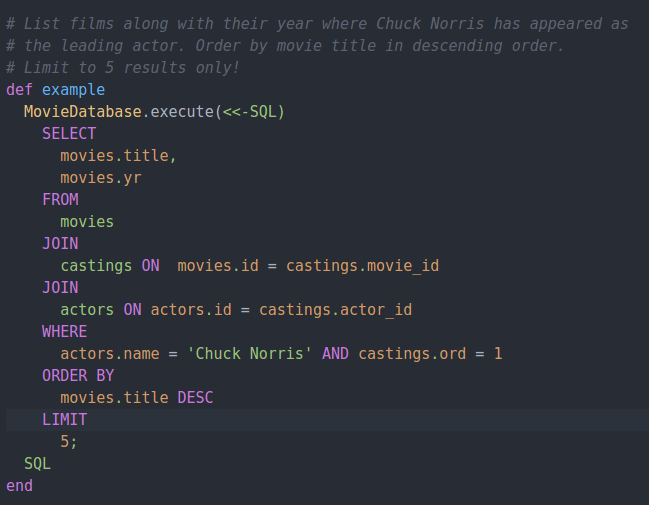
\includegraphics[width=13cm]{join.png}
                \end{center}
            \end{figure}

% Don't forget this line in order to increment the exercise counter
\nextexercice

%******************************************************************************%
%                                                                              %
%                             THE SQL PISCINE LOL                              %
%                                                                              %
%******************************************************************************%

\chapter{Day \exercicenumber: This is the end, isn't it? Nobody lives forever }
\extitle{DB creation!}
\exfiles{The entire folder where you've stored your DB, SQL queries, wrapper program, data files, etc}
\exnotes{Make sure to use docker cp to store your files on the host computer, then add it to a git repo after!}
\makeheaderfiles

            \begin{figure}[H]
                \begin{center}
                    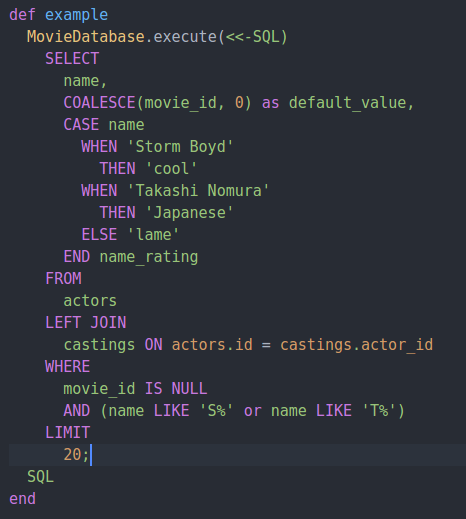
\includegraphics[width=9cm]{null.png}
                \end{center}
            \end{figure}

	\begin{itemize}\itemsep1pt
		\item	Further instructions on DB creation and clarification w/ images? -> They've had enough help!  
		\item	Mention Parseltongue course! Ways to get data: webscraping, APIs, manually enter, randomly generate
			Ex. of one of the methods used to get data in image below
		\item	Mention ORM and ask why we go for higher levels of abstraction 
		\item	Rec. to put everything in an object and have a consistent naming scheme. Ex. in image above
	\end{itemize}

	\begin{figure}[H]
		\begin{center}
			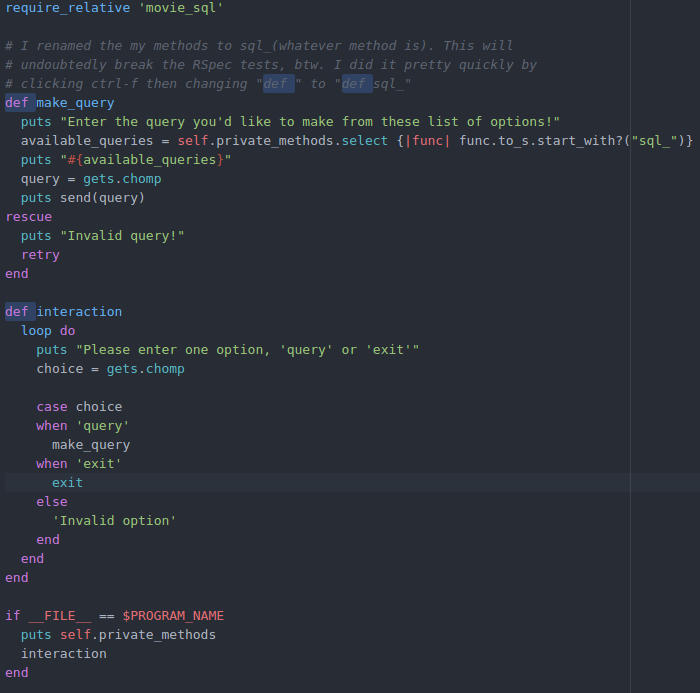
\includegraphics[width=15cm]{wrapper.png}
		\end{center}
	\end{figure}

% Don't forget this line in order to increment the exercise counter
\nextexercice


%******************************************************************************%
%                                                                              %
%                                 Bonus part                                   %
%                                                                              %
%******************************************************************************%
\chapter{Bonus part}
	Well, the first bonus is the same as the last project! It's simply to write your 
	own query questions, the solution to said questions, and a test to check if the 
	solution is correct. Write 5 of these and you'll get all the bonus points! \\ 

	If your material is good, it'll be added to the curriculum to make the 
	next gen of H2S SQL students suffer. The more work the better, right? \\ 

	Anyhow, the second bonus is much more fun. It's basically just adding extra 
	features to your wrapper program or making it look pretty. Something that would be 
	cool would be letting users interact with your database through a website or API. \\ 

	Oi oi, learn some Ruby on Rails from H2S and let's implement some good ol' MVC 
	architecture applications and websites. Or you could be lame and learn Flask instead! 

	\begin{figure}[H]
		\begin{center}
			
\includegraphics[width=12cm]{flask.png}
		\end{center}
	\end{figure}

%******************************************************************************%
%                                                                              %
%                           Turn-in and peer-evaluation                        %
%                                                                              %
%******************************************************************************%
\chapter{Turn-in and peer-evaluation}
    Turn your work in using your \texttt{GiT} repository, as
    usual. Only work present on your repository will be graded in defense. \\
	
	Remember to store all your work on a git repository-- make sure to add, commit, then push! \\ 

    Good luck and don't forget to "cd (where you stored your work) \&\& rm -rf *" once you're done.

    . \\

    . \\

    . \\ 

    . \\ 

    . \\ 

    . \\

    . \\

    . \\

    . \\
    
    . \\

    . \\
    
    . \\

    . \\

    If you've actually followed instructions and stored your work, you'll be fine.

%******************************************************************************%
\end{document}
